\chapter{Desarrollo}
\label{chap:desarrollo}

El desarrollo de este trabajo, se describe siguiendo la metodología planteada anteriormente. Las iteraciones citadas en el \textit{Marco Metodológico} serán descritas a continuación de manera consecutiva:

\section{[Iteración 1]: Investigación y análisis}
Durante esta etapa no se desarrolló ningún tipo de software, es por ello que no se verán historias de usuario, diseño, desarrollo ni pruebas unitarias.

\subsection{Desarrollo de las tareas}
Las tareas de esta iteración se basaron principalmente en la investigación y profundización de los temas relacionados a este trabajo, así como la búsqueda de herramientas para el ensamblaje de la plataforma de desarrollo.

\subsubsection{Investigación de los temas relacionados}
La mayor parte de la investigación realizada fue descrita en el \textit{Marco Teórico} del presente trabajo. El tópico central del presente trabajo resulta ser \textit{La Web Semántica}, por ello, es necesario tomar en cuenta todos los conceptos que se desprenden de dicho tópico. Los conceptos más importantes que se desprenden de \textit{La Web Semántica} son citados a continuación:

\begin{itemize}
\item Ontologías o modelos de conocimiento.
\item Motores de inferencia.
\item Servicios Web.
\end{itemize}

Las \textit{Ontologías} o \textit{Modelos de conocimiento}, son el marco central de la \textit{Web Semántica}. Es lo que establece toda la estructura de metadatos en la que se basa el etiquetado e indexado de los recursos que forman parte de la base de conocimientos. Además, establece las relaciones entre las metaentidades que conforman la \textit{Ontología}. Define el vocabulario que modela el dominio del problema a ser resuelto.

Los \textit{Motores de inferencia} son herramientas que, dadas ciertas reglas sobre un \textit{modelo de conocimiento}, son capaces de deducir nueva información y nuevas relaciones entre las metaentidades y, por lo tanto, nuevas relaciones entre los recursos dentro de la base de conocimientos.

Los \textit{Servicios Web}, si bien son un concepto que ya tiene tiempo, cobran especial importancia en la \textit{Web Semántica} pues, cuando se haga efectiva la evolución de la Web 2.0 a la Web 3.0, debe garantizarse total interoperabilidad e independencia de plataformas para que los agentes puedan ser capaces de consultar e intercambiar información y \textit{modelos de conocimiento} de distintas fuentes. Los \textit{servicios} web exponen toda la funcionalidad de un sistema a través de métodos invocables utilizando HTTP sobre TCP. Es por ello que, a través de \textit{Servicios Web}, es posible desarrollar servicios sobre cualquier plataforma y, sin importar en cual otra esté desarrollado, cualquier cliente será capaz de consumir los servicios pues la invocación se encapsula dentro de un protocolo común entre ambas plataformas.

\subsubsection{El problema y los requerimientos}
Del problema general del proyecto, puede plantearse de la siguiente manera: \textit{¿Cómo facilitar el acceso a la información acerca de Ciencias de la Computación a personas interesadas en el área?}. De este problema, puede identificarse los siguientes requerimientos:

\begin{itemize}
\item Una interfaz web donde los usuarios puedan interactuar con el sistema.
\item Una interfaz de edición que permita a usuarios autorizados agregar nuevos recursos y extender la base de conocimiento.
\item Una interfaz de edición que permita a usuarios autorizados agregar metainformación nueva y extender el modelo de conocimiento.
\item Un componente de traducción que convierta consultas en lenguaje natural a SPARQL, el lenguaje de consultas sobre RDF/RDFS/OWL.
\item Desarrollo de un modelo de conocimiento del área de Ciencias de la Computación e Ingeniería Informática.
\item Un componente capaz de realizar consultas e inferencias sobre el modelo de conocimiento realizado.
\end{itemize}

\subsubsection{Selección de la plataforma}
Al ser una aplicación bajo la arquitectura Cliente-Servidor, hay que tener especial cuidado en seleccionar las mejores herramientas para desarrollar cada uno de los componente de dicha arquitectura.

Al principio, se planteó llevar a cabo todo el desarrollo utilizando \textit{Python} como lenguaje de programación y las librerías nativas disponibles a través de \textit{easy\_install}, pues \textit{Python} es uno de los pocos lenguajes que ofrece librerías nativas para la manipulación de documentos RDF, además de las ventajas propias que ofrece el lenguaje desde el punto de vista sintáctico y de facilidad de aprendizaje y de programación. Pero a la hora de buscar Frameworks que permitieran el desarrollo de aplicaciones basadas en Web Semántica y Motores de Inferencia, la información y la cantidad de herramientas resultó limitada.

Debido a la situación expuesta en el párrafo anterior, se planteó evaluar el desarrollo por separado: seleccionar la mejor plataforma para desarrollar el servidor y, por otra parte, la mejor plataforma para desarrollar el cliente:

\subsubsection{Servidor}
Las dos opciones más fuertes para el desarrollo del lado del Servidor fueron \textit{Python} por un lado, por ser una plataforma 100\% libre y de código abierto y por la gran cantidad de librerías disponibles para extender el lenguaje, y por otro lado \textit{Java} representaba una opción viable, por ser una plataforma con más de 15 años de desarrollo y estándar \textit{de-facto} de la industria, a continuación se presentan las características más destacables de cada una de las opciones:

\begin{itemize}
\item \textbf{Python[17]:}
    \begin{itemize}
    \item Totalmente abierto y libre.
    \item Sintaxis clara y legible.
    \item Capacidad poderosa de introspección.
    \item Multiparadigma: funcional, estructurado y orientado a objetos.
    \item Tipos de dato dinámicos.
    \item Gestión de errores basada en excepciones.
    \item Puede extenderse a través de la escritura de módulos en lenguaje C o C++.
    \item Gran cantidad de librerías, entre ellas varias para procesar documentos RDF.
    \item Facilidad para interoperar con otras plataformas.
    \item Precompilado y semi-interpretado.
    \end{itemize}
\item \textbf{Java[18]:}
    \begin{itemize}
    \item Sencillo, fue diseñado para facilitar las tareas del programador profesional.
    \item Orientado a objetos.
    \item Distribuido, facilita el desarrollo de aplicaciones que hacen uso de la red mediante la incorporación de clases que manejan protocolos TCP/IP.
    \item Precompilado y semi-interpretado.
    \item Arquitectura neutra, debido a que se ejecuta en una máquina virtual.
    \item Portable, dado que al ``compilar" no se produce un archivo ejecutable como ocurre en los lenguajes compilados (como C, C++ y Pascal, por ejemplo), sino un \textit{bytecode} que es ejecutado por la máquina virtual, este \textit{bytecode} puede ser ejecutado en cualquier otro sistema operativo, siempre y cuando exista en él una instancia de la \textit{Máquina Virtual de Java}.
    \item Multihilo, un programa en \textit{Java} puede ejecutar múltiples tareas de manera simultánea
    \end{itemize}
\end{itemize}

Ambas plataformas ofrecen prestaciones muy similares, si bien el núcleo de \textit{Python} no es muy amplio, posée gran cantidad de librerías para extender su funcionalidad. De igual manera, \textit{Java} incorpora cientos de clases que lo convierten en un lenguaje amplio y poderoso.

Para el servidor, se decidió trabajar con \textit{Java}, ya que, como se verá más adelante, ofrece el mejor framework para el desarrollo de aplicaciones basadas en Web Semántica y, al seleccionar dicho framework, la transitividad nos lleva a trabajar con este lenguaje.

\subsubsection{Cliente}
El cliente, es el encargado de realizar peticiones al servidor e interactuar con el usuario final, es por ello que la generación de vistas es un aspecto importante en esta parte del sistema.

Para el desarrollo del cliente, fue seleccionada la plataforma \textit{Python}, debido a todas las razones expuestas anteriormente.

\subsubsection{Selección de los frameworks de desarrollo}
Luego de realizar una investigación en la web, los frameworks de desarrollo que parecen ser más utilizados para las aplicaciones semánticas son:

\begin{itemize}
    \item \textbf{Sesame:} escrito en \textit{Java}.
    \item \textbf{RedLand:} escrito en C y accesible desde \textit{Python} mediante \textit{Wrapping}.
    \item \textbf{Jena:} escrito en \textit{Java}.
    \item \textbf{CubicWeb:} escrito en \textit{Python}.
\end{itemize}

En este caso, se tomó la decisión de trabajar con el framework \textit{Jena} debido a que es el que ofrece la mayor cantidad de documentación disponible en línea, además, es compatible con todos los niveles de representación semántica de metainformación (RDF, RDFS y OWL), posée varios motores de inferencia ya integrados y permite la integración con motores de inferencia externos, tiene un motor de consultas SPARQL y ofrece la posibilidad de integrarse con medios de persistencia externos, además de ser libre y de código abierto[19].

El framework \textit{Sesame}, ofrece prestaciones técnicas similares a las de \textit{Jena}, sin embargo, la documentación disponible en línea no es comparable con la que ofrece este último y, a pesar de ser de código abierto, es propiedad de una empresa alemana llamada \textit{ADUNA}[20] y para poder acceder a información más profunda o solicitar ayuda en algo relacionado al framework, es necesario pagar por horas de consultoría, lo que hace poco viable la utilización de \textit{Sesame} para este proyecto.

\textit{RedLand}, escrito en C y accesible desde \textit{Python}, luego de leer la documentación, es compatible sólo con RDF y, para este trabajo, el modelo de conocimientos planteado utilizaría anotaciones definidas en la especificación RDFS y, posiblemente, algunas definidas en el dialecto OWL-Lite, popr lo que fue descartado. Además, el proceso de instalación y configuración resulta complicado comparado al de las otras opciones[21].

Finalmente \textit{CubicWeb}, a pesar de ser un framework realmente completo pues ofrece toda la plataforma para el desarrollo: desde la persistencia, hasta la generación de vistas, pero fue descartado por no ser compatible con SPARQL, sino con su antecesor: RQL[22].

\subsubsection{Selección del medio de persistencia}
Para la persistencia de datos, si bien los manejadores de base de datos relacionales tradicionales como MySQL y Postgres ofrecen paquetes para la gestión de documentos RDF y OWL, existe una alternativa que ofrece dicha funcionalidad de manera nativa. Se trata de \textit{Virtuoso}, un manejador de base de datos con capacidad de gestionar información en formato RDF y XML, compatible con los estándares ODBC y JDBC, posée un motor de inferencia interno, puede correr en ambientes federados[23] y, además, exite una edición \textbf{Open Source} bastante completa y muy bien documentada.

\section{[Iteración 2]: Diseño de la arquitectura del sistema}


\section{[Iteración 3]: Establecimiento del ambiente de desarrollo}
En esta iteración no se desarrolló ningún tipo de software, por ello, no se fue necesaria la realización de pruebas unitarias, sin embargo, se llevó a cabo un proceso de configuración posterior a la selección de las herramientas de desarrollo.

\subsection{Desarrollo de las tareas}
El proceso que dirigirá la etapa de desarrollo, será el proceso de programación o codificación, en dos lenguajes de programación distintos: \textit{Python} del lado del \textit{Cliente} y \textit{Java} del lado del \textit{Servidor}, es por ello que el \textit{Sistema Operativo} utilizado en el equipo de desarrollo y despliegue del sistema, \textbf{debe} facilitar la instalación y configuración de las herramientas necesarias para realizar dicho trabajo, además de albergar el sistema una vez desarrollado.

A nivel de \textit{Sistema Operativo}, se seleccionó una distribución de \textit{GNU/Linux}, muy popular en el mundo de los desarrolladores de software y servidores, ya que ofrece compatibilidad con \textit{Java} a través de una instancia de la máquina virtual y el intérprete de \textit{Python} usualmente viene preinstalado en todos los sistemas \textit{GNU/Linux}. La distribución seleccionada fue \textit{Debian} pues, ofrece alrededor de 30.000 paquetes de software instalables a través del gestor de paquetes \textit{aptitude} o, su front-end gráfico \textit{Synaptic}[23], además, las versiones de esta distribución de \textit{GNU/Linux} usualmente tienen años de diferencia pues la comunidad pone especial atención en liberar software que está 100\% probado y estable[24].

A nivel de servidores de aplicaciones, se seleccionó \textit{Jetty} para alojar la aplicación \textit{servidora}, ya que es recomendado por la misma comunidad de \textit{Jena} y \textit{Apache2} para alojar la aplicación \textit{cliente}, junto con \textit{libapache-mod-python} para activar la compatibilidad del servidor \textit{Apache2} con \textit{Python}.

Para desarrollar las tareas de programación, se seleccionaron las siguientes herramientas:
\begin{itemize}
    \item Para desarrollar en \textit{Java}, se seleccionó el Entorno Integrado de Desarrollo (IDE) \textit{Eclipse}
    \item La \textit{Ontología}, ya que debe ser escrita en RDF/OWL, se seleccionó el editor \textit{Protègè}, desarrollado en la Universidad de Stanford, este editor, permite el modelado de manera gráfica y la generación automática de código válido en varias sintaxis de RDF/OWL.
    \item Para desarrollar en \textit{Python}, los requerimientos no son muchos, por ello, para mantenerlo simple, se seleccionó el editor \textit{VIM}, con los siguientes \textit{plugins}:
    \begin{itemize}
        \item NERDTree, que permite la visualización de la estructura de directorios del proyecto y la apertura de varios archivos de código fuente en distintas pestañas a nivel de terminal.
        \item PyDiction, un diccionario de \textit{Python} para facilitar el autocompletado y autocorrección de código fuente.
    \end{itemize}
\end{itemize}

\subsubsection{Configuración}
%TODO: redactar aquí cómo fue configurado el ambiente

\section{[Iteración 4] Análisis y desarrollo de la \textit{ontología}}
Durante esta iteración, si bien se desarrolló una parte importante del sistema como lo es la \textit{ontología}, no se codificó software como tal. La etapa de pruebas unitarias, fue sustituída por una etapa de validación del modelo de conocimiento.

\subsection{Desarrollo de las tareas}
Para el desarrollo de la \textit{ontología} definitiva, fue necesario realizar un análisis previo para determinar cómo está estructurado el conocimiento en las áreas de \textit{Ciencias de la Computación} e \textit{Ingeniería Informática}, posteriormente, se procedió a realizar el diseño, codificación y validación de la \textit{ontología} hata llegar al modelo final.

\subsubsection{Análisis}
Antes de realizar un diseño preliminar de la \textit{ontología}, es necesario realizar un análisis de la estructura del conocimiento en el área, con este análisis se busca:

\begin{enumerate}
    \item Establecer las \textit{entidades} que conformarán la \textit{ontología}.
    \item Determinar las \textit{relaciones} existentes entre las \textit{entidades}.
    \item Conocer más a fondo el dominio del problema a ser resuelto.
\end{enumerate}

Los tres (3) ítems enumerados anteriormente, pueden resumirse como \textit{Determinar la estructura del conocimiento en el área seleccionada}. Para ello, es necesario aplicar técnicas de \textit{Ingeniería del Conocimiento}. Un \textit{Ingeniero de Conocimiento}, es alguien que investiga un dominio concreto, aprende qué conceptos son los importantes de ese dominio y crea una representación formal de los objetos y relaciones del dominio[25]. En este caso, el dominio ya ha sido investigado por el autor durante los años de carrera, simplemente hace falta determinar qué conceptos son importantes en el área y producir la representación formal de dichos conceptos y las relaciones que guardan entre sí.

\subsubsection{Diseño}
%TODO: decidir si coloco los documentos en bibliografía o si los referencio como apéndices
Luego de analizar el área seleccionada y con base en las recomendaciones de la \textit{IEEE Computer Sociery} (IEEE-CS) y la \textit{Assosiation for Computing Machinery} (ACM), descritas en los documentos \textit{Computing Curricula 2001, Computer Science Final Report} para el campo de las \textit{Ciencias de la Computación} y el documento \textit{Computer Engineering 2004: Curriculum Guidelines for Undergraduate Programs in Computer Engineering}, que incorpora elementos de Ingeniería al primero, se llegó a la estructura jerárquica de clases mostrada en la  Figura~\ref{classHierarchy}:

\newpage

\begin{figure}
    \begin{center}
        \label{classHierarchy}
        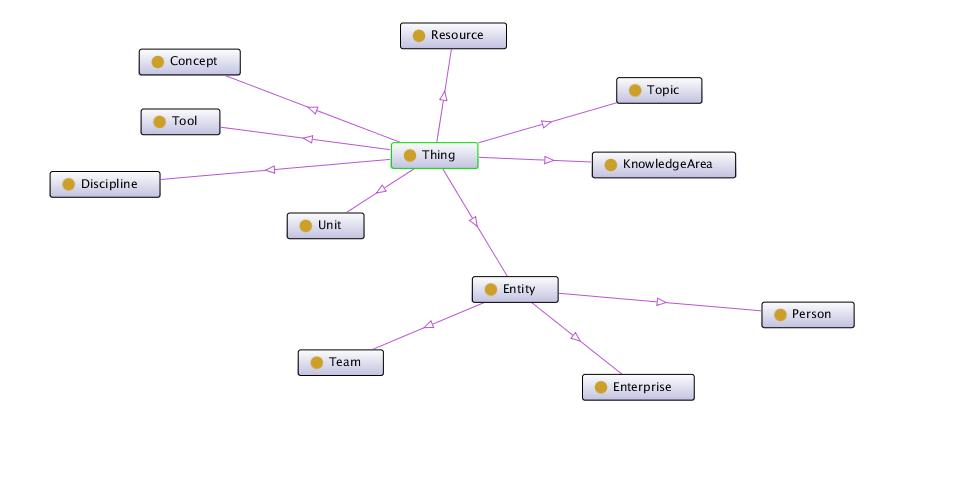
\includegraphics[scale=0.5]{/home/israelord/Dissertation/Book/my_files/images/onto_graph_classes.jpg}
        \caption{Jerarquía de clases}
    \end{center}
\end{figure}

En RDF/OWL, todas las clases o entidades heredan por defecto de la clase \textit{Thing}, un principio similar al de la clase \textit{Object} en \textit{Java}, las líneas moradas expresan precisamente eso, una relación de \textit{herencia} entre dos entidades que puede leerse como \textit{is-a} (\textit{es-un} o \textit{es-una}), esta relación de \textit{herencia} es, además, transitiva, lo que nos permite inferir, por ejemplo, que un elemento de la clase \textit{Person}, es también un \textit{Thing} aunque no exista una relación directa, pues la clase de nivel inmediatamente superior lo es. Las clases \textit{KnowledgeArea}, \textit{Unit} y \textit{Topic}, son las mismas utilizadas en los documentos de la \textit{IEEE-CS} y la \textit{ACM} para dividir los grandes bloques de conocimiento, en unidades más pequeñas, manejables y específicas a cada nivel como se muestra en la Figura~\ref{knowledgeStructure}. La clase \textit{Discipline}, fue agregada para hacer referencia al marco global del problema cuyo dominio se está modelando, en este caso \textit{Ciencias de la Computación}, con el objetivo de facilitar la adaptación de este modelo a otros dominios. Por otra parte, la clase \textit{Concept}, fue agregada con el propósito de lograr una granularidad más fina y poder expresar niveles de conocimiento más específico, las clases \textit{Entity}, \textit{Person}, \textit{Team} y \textit{Enterprise} serán explicadas posteriormente.
\newpage

\begin{figure}
    \begin{center}
        \label{knowledgeStructure}
        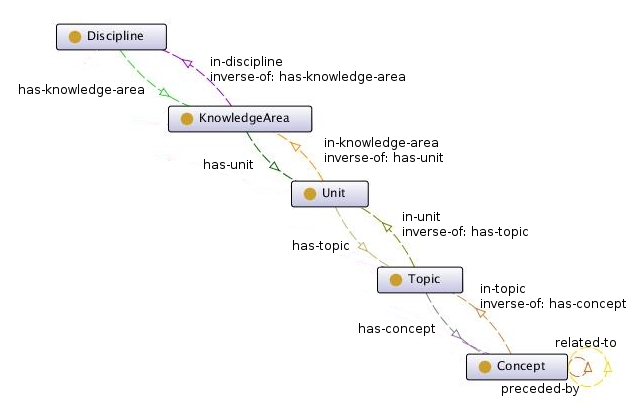
\includegraphics[scale=0.5]{/home/israelord/Dissertation/Book/my_files/images/onto_knowledge_structure.jpg}
        \caption{Estructura del conocimiento según \textit{IEEE-CS} y \textit{ACM}}
    \end{center}
\end{figure}

En la Figura~\ref{knowledgeStructure} se muestra la estructura del conocimiento según las recomendaciones de la \textit{ACM} y la \textit{IEEE-CS}, puede observarse que es una estructura de \textit{Contención}, donde el nivel superior engloba todo lo que se encuentra en los niveles inferiores. También, según la Figura~\ref{knowledgeStructure}, las propiedades a la derecha (las que tienen el prefijo \textit{in}) son propiedades inversas de las de la izquierda (las que tienen el prefijo \textit{has}). Anotar esas propiedades como inversas, permite que a la hora de declarar un \textit{Named Individual} (instancias) en alguna de las clases, sólo sea necesario especificar una de las dos propiedades. Toda la estructura de contención va desde la clase más general (\textit{Discipline}) que contiene a toda la estructura, hasta la clase más específica (\textit{Concept}) que es el último eslabón de la cadena. Sólo con las relaciones descritas anteriormente y representadas de manera gráfica en la Figura~\ref{knowledgeStructure}, no basta para expresar lo dicho anteriormente pues ninguno de los atributos dibujados es transitivo, además, son propiedades distintas y no expresan ningún tipo de significado una de la otra sino que tienen significado por sí solas. Para solventar esta situación, se crearon dos súper-propiedades: \textit{contents} y \textit{content-by}, ambas transitivas e inversas una de la otra y que envuelven las propiedades \textit{has} e \textit{in} respectivamente.

De esta manera, además de lo descrito en la Figura~\ref{knowledgeStructure}, queda expresada la \textit{Jerarquía de Contención} mostrada en la Figura~\ref{contentHierarchy} gracias a la propiedad \textit{contents}:

\begin{figure}[h]
    \begin{center}
        \label{contentHierarchy}
        \textit{Discipline} \subseteq \textit{KnowledgeArea} \subseteq \textit{Unit} \subseteq \textit{Topic} \subseteq \textit{Concept}
        \caption{Jerarquía de Contención}
    \end{center}
\end{figure}

De la misma manera, también, a través de su relación inversa \textit{content-by}, queda expresado lo descrito en la Figura~\ref{inverseContentHierarchy}

\begin{figure}[h]
    \begin{center}
        \label{inverseContentHierarchy}
        \textit{Discipline} \supseteq \textit{KnowledgeArea} \supseteq \textit{Unit} \supseteq \textit{Topic} \supseteq \textit{Concept}
        \caption{Jerarquía de Contención Iversa}
    \end{center}
\end{figure}

En la Figura~\ref{knowledgeStructure}, se observan dos relaciones recursivas en le entidad \textit{Concept}, estas son: \textit{related-to} y una sub-propiedad \textit{preceded-by}, estas propiedades son \textit{simétrica} y \textit{transitiva} respectivamente, con esta jerarquía de propiedades, se expresa que si un concepto \textit{precede} a otro, entonces, también están \textit{relacionados}.



\newpage
